% Auto-generated by 04_additional_analysis.R — do not edit
% y > 0: Underreacts  |  y < 0: Overreacts
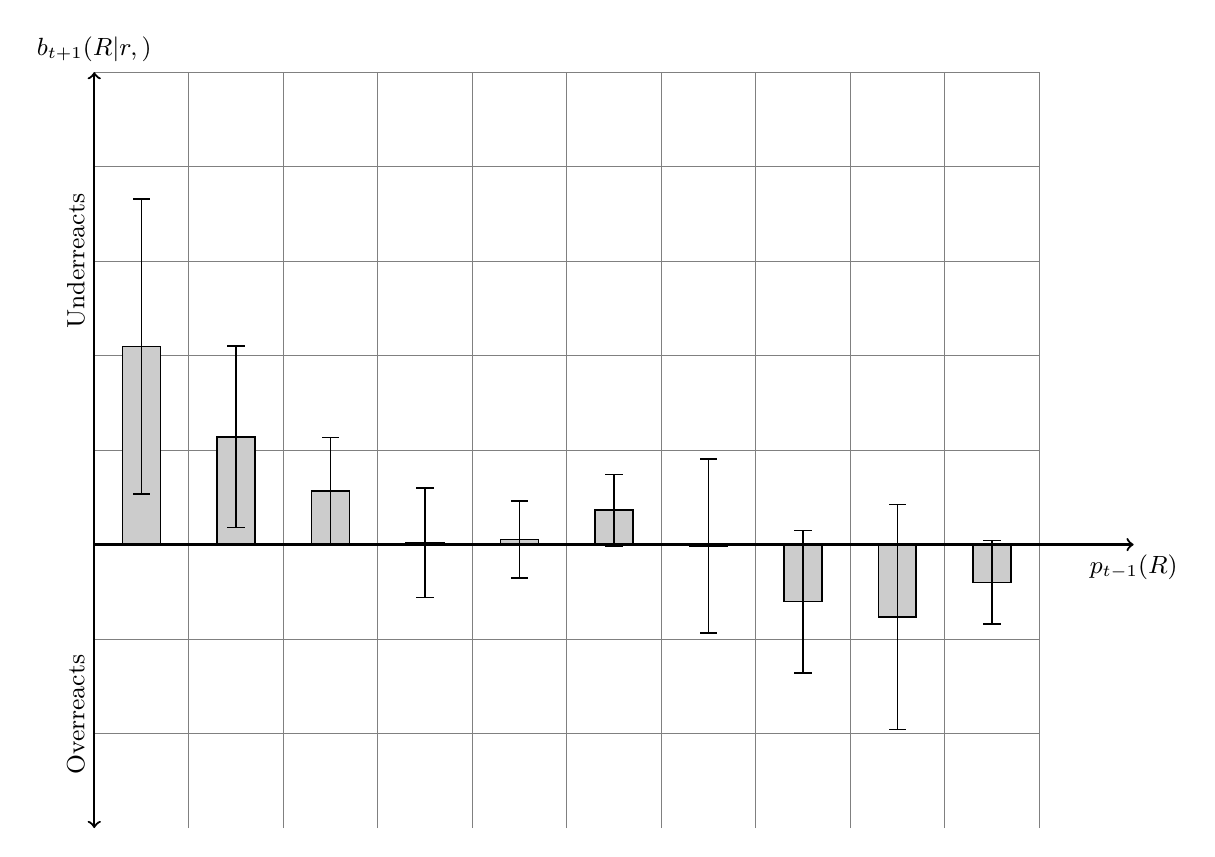
\begin{tikzpicture}[scale=12]
\draw[help lines,step=0.1] (0,-0.3) grid (1,0.5);
\filldraw[opaque,white!80!black] (0.03,0) rectangle (0.07,0.2095);
\draw[line width=0.6] (0.03,0) rectangle (0.07,0.2095);
\draw[line width=0.6,|-|] (0.05,0.0524) -- (0.05,0.3666);
\filldraw[opaque,white!80!black] (0.13,0) rectangle (0.17,0.1140);
\draw[line width=0.6] (0.13,0) rectangle (0.17,0.1140);
\draw[line width=0.6,|-|] (0.15,0.0171) -- (0.15,0.2109);
\filldraw[opaque,white!80!black] (0.23,0) rectangle (0.27,0.0570);
\draw[line width=0.6] (0.23,0) rectangle (0.27,0.0570);
\draw[line width=0.6,|-|] (0.25,-0.0003) -- (0.25,0.1143);
\filldraw[opaque,white!80!black] (0.33,0) rectangle (0.37,0.0021);
\draw[line width=0.6] (0.33,0) rectangle (0.37,0.0021);
\draw[line width=0.6,|-|] (0.35,-0.0570) -- (0.35,0.0611);
\filldraw[opaque,white!80!black] (0.43,0) rectangle (0.47,0.0053);
\draw[line width=0.6] (0.43,0) rectangle (0.47,0.0053);
\draw[line width=0.6,|-|] (0.45,-0.0364) -- (0.45,0.0469);
\filldraw[opaque,white!80!black] (0.53,0) rectangle (0.57,0.0365);
\draw[line width=0.6] (0.53,0) rectangle (0.57,0.0365);
\draw[line width=0.6,|-|] (0.55,-0.0023) -- (0.55,0.0752);
\filldraw[opaque,white!80!black] (0.63,0) rectangle (0.67,-0.0013);
\draw[line width=0.6] (0.63,0) rectangle (0.67,-0.0013);
\draw[line width=0.6,|-|] (0.65,-0.0943) -- (0.65,0.0916);
\filldraw[opaque,white!80!black] (0.73,0) rectangle (0.77,-0.0604);
\draw[line width=0.6] (0.73,0) rectangle (0.77,-0.0604);
\draw[line width=0.6,|-|] (0.75,-0.1366) -- (0.75,0.0158);
\filldraw[opaque,white!80!black] (0.83,0) rectangle (0.87,-0.0767);
\draw[line width=0.6] (0.83,0) rectangle (0.87,-0.0767);
\draw[line width=0.6,|-|] (0.85,-0.1965) -- (0.85,0.0432);
\filldraw[opaque,white!80!black] (0.93,0) rectangle (0.97,-0.0400);
\draw[line width=0.6] (0.93,0) rectangle (0.97,-0.0400);
\draw[line width=0.6,|-|] (0.95,-0.0851) -- (0.95,0.0051);
\draw[line width=0.8,->]  (0,0) -- (1.1,0) node[below] {\small{$p_{t-1}(R)$}};
\draw[line width=0.8,<->] (0,-0.3) -- (0,0.5) node[above] {\small{$b_{t+1}(R|r,\xmark)$}};
\draw (0,0.30) node[above,rotate=90] {\small{Underreacts}};
\draw (0,-0.18) node[above,rotate=90] {\small{Overreacts}};
% ADD THEORY CURVE BELOW
\end{tikzpicture}
